\documentclass[11pt,letter]{moderncv}

\moderncvtheme[grey]{casual}

\usepackage[margin=1in]{geometry}

\usepackage{background}

\usepackage{tkz-graph}
\usetikzlibrary{arrows,shapes,decorations.markings}

\tikzstyle{every picture}+=[
  xnode/.style={fill=gray!20,shape=rectangle,draw},
  ynode/.style={fill=white!100,shape=circle,draw},
  enode/.style={fill=white!100,shape=rectangle,draw}
]

\newcommand*{\cyccwl}[2][.5cm]{\draw[decoration={markings, mark=at position .5 with {\arrowreversed{triangle 90}}}, postaction={decorate}] #2 circle (#1)}

\newcommand*{\cycccwl}[2][.5cm]{\draw[decoration={markings, mark=at position .5 with {\arrow{triangle 90}}}, postaction={decorate}] #2 circle (#1)}

\newcommand*{\cyccwr}[2][.5cm]{\draw[decoration={markings, mark=at position 0 with {\arrowreversed{triangle 90}}}, postaction={decorate}] #2 circle (#1)}

\newcommand*{\cycccwr}[2][.5cm]{\draw[decoration={markings, mark=at position 0 with {\arrow{triangle 90}}}, postaction={decorate}] #2 circle (#1)}

\backgroundsetup{
  color=black!12,
  scale=4,
  angle=-47,
  hshift=-15,
  vshift=-7,
  contents={
    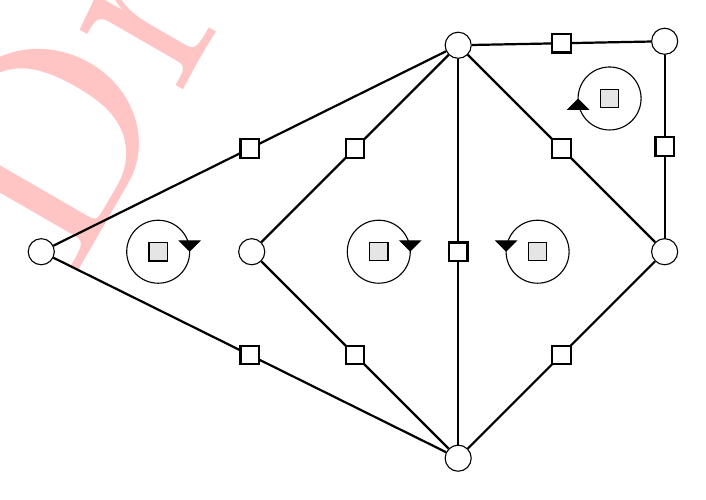
\begin{tikzpicture}
      \def\nodesep{2.5cm}
      \def\cycrad{0.4cm}
      \node[style=ynode] (a) at (0, 0) {};
      \node[style=ynode,above left = \nodesep] at (a) (d) {};
      \node[style=ynode,above right = \nodesep] at (a) (f) {};
      \node[style=ynode,above right = \nodesep] at (d) (c) {};
      \node[style=ynode,left = \nodesep] at (d) (b) {};
      \node[style=ynode,above = \nodesep] at (f) (e) {};
      %
      \path [draw, thick] (a) to node[style=enode] (4) {} (c);
      \path [draw, thick] (a) to node[style=enode] (9) {} (f);
      \path [draw, thick] (a) to node[style=enode] (2) {} (d);
      \path [draw, thick] (a) to node[style=enode] (1) {} (b);
      \path [draw, thick] (b) to node[style=enode] (6) {} (c);
      \path [draw, thick] (d) to node[style=enode] (5) {} (c);
      \path [draw, thick] (f) to node[style=enode] (3) {} (c);
      \path [draw, thick] (c) to node[style=enode] (8) {} (e);
      \path [draw, thick] (f) to node[style=enode] (7) {} (e);
      %
      \node [style=xnode] (A) at (barycentric cs:f=1,c=1,e=1.75) {};
      \node [style=xnode] (B) at (barycentric cs:a=1,d=1.25,c=1) {};
      \node [style=xnode] (C) at (barycentric cs:a=1,c=1,f=1.25) {};
      \node [style=xnode] (D) at (barycentric cs:b=1,d=1.25) {};
      %
      \cyccwl[\cycrad]{(A)};
      \cyccwr[\cycrad]{(B)};
      \cycccwl[\cycrad]{(C)};
      \cyccwr[\cycrad]{(D)};
      %
    \end{tikzpicture}
  }
}

\usepackage{kpfonts}
\renewcommand{\sfdefault}{\rmdefault}

\firstname{Andrew}
\familyname{Gainer-Dewar}
\address{One North College Street}{Northfield, MN 55057}
\phone{(507) 222 4482}
\email{againerdewar@carleton.edu}

\begin{document}
\maketitle

\section{Education}
\cventry{2007--2012}{Ph.D.\ (Mathematics)}{Brandeis University}{Waltham}{MA}{}

\cventry{2003--2007}{B.S.\ (Mathematics) \& B.A.\ (Philosophy)}{Mercer University}{Macon}{GA}{}

\section{Professional appointments}
\cventry{2012--2014}{Visiting asst.\ prof.\ of mathematics}{Carleton College}{Northfield}{MN}{}

\section{Teaching}
\cventry{2012--2014}{Carleton College}{}{}{}{
  Calculus I, Calculus II, Linear Algebra, Advanced Linear Algebra (major-level)
}
\cventry{2008--2010}{Brandeis University (graduate instructor)}{}{}{}{
  Precalculus, Calculus I, Calculus II, Linear Algebra
}

%Publications section (header added by \bibliography)
\nocite{*}
\bibliographystyle{publist/utphys}
\bibliography{publist/publist}

\section{Undergraduate research supervised}
\cventry{2012}{On the species of bipartite point-determining graphs}{Carleton College}{}{}{}

\section{Presentations and talks}
\cventry{Feb.\ 2013}{Making strategy count: combinatorial game theory and the surreal numbers}{}{}{}{}

\cventry{Jan.\ 2013}{$\Gamma$-species and the enumeration of \boldmath{$k$}-trees}{}{}{}{}

\cventry{2012}{Contemporary graph enumeration and \boldmath{$k$}-trees}{}{}{}{}

\cventry{2012}{Arrow's Theorem and the impossibility of democracy}{}{}{}{}

\cventry{2011}{Categorial combinatorics and the theory of species}{}{}{}{}

\cventry{2007}{Piecewise-linear boundaries of surfaces that immerse isometrically in $\mathbf{R}^2$}{}{}{}{}

\section{Service}
\cventry{January 2013}{JMM Undergraduate Poster Session Judge}{}{}{}{}
\cventry{2012--}{Department social co-coordinator}{Carleton}{}{}{}
\cventry{2012--}{Math GRE preparation co-coordinator}{Carleton}{}{}{}
\cventry{2008--2012}{Graduate student representative and social coordinator}{Brandeis}{}{}{}
\end{document}
